\appendix
\pagenumbering{Roman}

\newappendix{Získávání snímků obrazovky z~digitálního osciloskopu Agilent~54621A}
Autorův digitální osciloskop Agilent~54621A má poškozenou disketovou mechaniku,
proto není možné využít standardní metody získávání snímků obrazovky
a~textových dat. Pro účely tvorby dokumentace pro tuto práci byl vyvinut
jednoduchý počítačový program umožňující čtení obrázků ve formátu BMP přes
sériový port RS-232.

Je potřeba použít RS-232 kabel zapojený podle diagramu v dokumentaci
osciloskopu.

\begin{figure}[htbp]
    \centering
    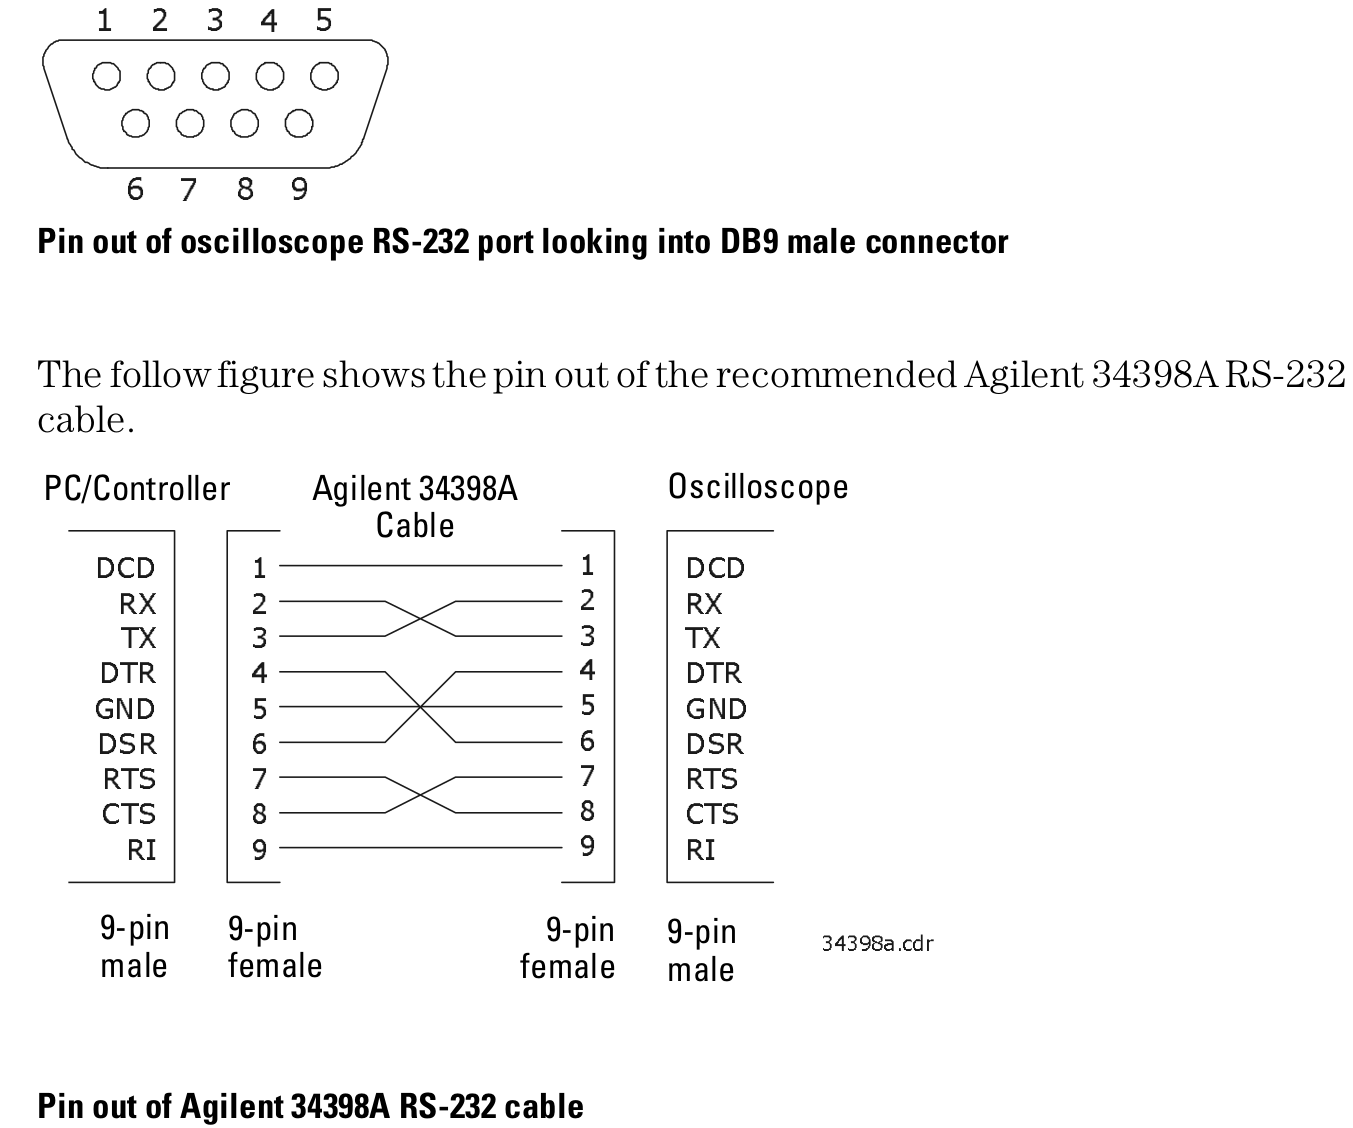
\includegraphics[width=\textwidth]{Agilent-RS232-pinout}
    \caption{%
        Zapojení kabelu pro propojení osciloskopu Agilent~54621A
        s~počítačem~\cite{Agilent54621Auser}
    }
    \label{fig:agilent RS232 pinout}
\end{figure}

Program napsaný v jazyce Python je uložen v souboru \filename{scrot}:
\lstinputlisting[language=Python,style=numbers]{prilohy/scrot}

Příklad použití v prostředí operačního systému GNU/Linux:
\begin{lstlisting}[style=terminal]
$ ./scrot -h
usage: scrot [-h] device file

positional arguments:
  device      Serial port the scope is attached to
  file        File to write the output to

optional arguments:
  -h, --help  show this help message and exit

$ ./scrot /dev/ttyUSB1 nazev-souboru
TODO scrot vystup + ls -l
\end{lstlisting}


% TODO prilohy
